\begin{wrapfigure}{r}{0.4 \textwidth}
  \begin{center}
    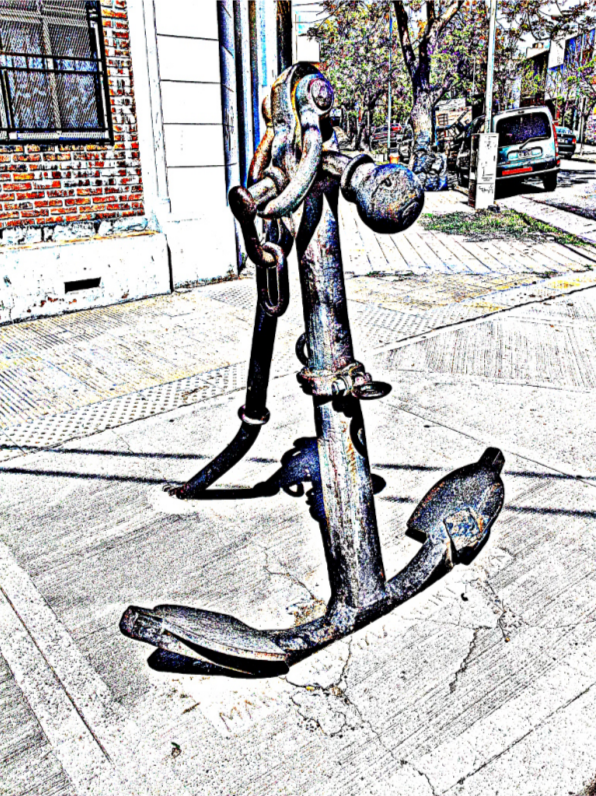
\includegraphics[scale=0.15]{imagenes/ancla.png}
  \end{center}
  \caption{Ancla}
\end{wrapfigure}
\par{
\section{Conclusión}
\bigskip
\subsection{Ancla}
}
\textcolor{white}{.}\\
\\
\bigskip
Queremos aportar a la cátedra nuestro siguiente descubrimiento: \\ 
Respondiendo al punto optativo \textbf{4.8 inciso d}, el ancla de la siguiente imagen, misma imagen que la figura 2 del enunciado del TP; se encuentra en la esquina de la intersección de las calles Pedernera y Tte. Cnel. Casimiro Recuero en el barrio porteño de Flores.

\bigskip
\bigskip
\bigskip
\bigskip
\bigskip
\subsection{Ejercicio 4.8}
\par{
Luego de implementar lo descrito en este informe, sumado a ciertas funciones para imprimir en pantalla, creemos que nuestro sistema operativo cumple con lo establecido en el TP. Sin ir más lejos nos sentimos preparados y ansiosos por consagrarnos victoriosos del evento "Guerra de Tareas", ya que un navío letal está siendo diseñado para dicho propósito.}